\documentclass[a4paper, 14pt, oneside]{extbook}
\usepackage[T1]{fontenc}
\usepackage[utf8x]{inputenc}
\usepackage{geometry}
\usepackage{courier}
\usepackage[bookmarks]{hyperref}
\usepackage[italian]{babel}

\newgeometry{
left=   1.5 in,
bottom= 1.5 in,
right=  1 in,
top=    1 in
}

\usepackage{fancyhdr}

% Grafica
\usepackage{graphicx,pstricks}
\usepackage{graphics}
\graphicspath{{img/}}

% Package usati per il frontespizio
\usepackage{tikz}
\usepackage{pgf-pie}
\usepackage{pgfplots}
\pgfplotsset{width=7cm,compat=1.8}
\usetikzlibrary{patterns}


%Algorithm
\usepackage{algorithm}
\usepackage[noend]{algpseudocode}

\setlength\headheight{44.2pt}
%Page Style
\usepackage{setspace}
%\setstretch{2.5}
\doublespacing

%\cfoot{\thepage}
\lhead[]{}
\rhead[]{\leftmark}

\pagestyle{fancy}{
\lhead{
\includegraphics[scale=0.3]{img/logo/hlogo.png}}
\rhead{\footnotesize{Titolo abbreviato come intestazione}}
}

%Other
\usepackage{comment}
\usepackage{amsmath}

%Titolo indice
\renewcommand*\contentsname{Indice}

%Inclusione bibliografia nell'indice
\renewcommand\bibname{Bibliografia}
\usepackage[nottoc,notlot,notlof]{tocbibind}

\usepackage[noabbrev]{cleveref}

\crefformat{section}{\S#2#1#3}
\crefformat{subsection}{\S#2#1#3}
\crefformat{subsubsection}{\S#2#1#3}
\crefformat{figure}{#2Figura~#1#3}
\crefformat{footnote}{#2\footnotemark[#1]#3}
\crefformat{table}{#2Tabella~#1#3}
\crefformat{equation}{#2Equazione~#1#3}
\crefformat{chapter}{#2Capitolo~#1#3}


\begin{document}

%\maketitle
\begin{titlepage}
\thispagestyle{empty}
\raggedright % Allinea a sinistra

\begin{tikzpicture}
\node[anchor=south west] at (4,0) {
\includegraphics[scale=0.75]{img/logo/logo_copertina_1}};
\node[anchor=south west] at (0,1.5) {
\includegraphics{img/logo/logo_copertina_2}};
\node[anchor=south west] at (0,0.5) {\textsf{Scuola Politecnica e delle Scienze di Base}};
\node[anchor=south west] at (0,0) {\textsf{Corso di Laurea in Ingegneria Informatica}};
\end{tikzpicture}

\vfill

{\large Elaborato finale in Sistemi Operativi}
\\[1cm]
{\textbf{\textit{\LARGE Analisi delle prestazioni di scheduling a priorità}}}
\\[1cm]
{\large Anno Accademico 2021-2022}

\vfill


\begin{table}[h]
{\raggedright Candidato}
\\
\textbf{Giuseppe Capasso}
\\
\textbf{matr. N46003195}
\end{table}

\end{titlepage}
\frontmatter

\cleardoublepage
%\thispagestyle{empty}
\vspace*{\stretch{1}}
\begin{flushright}
\itshape Ad Angela, la mia persona arancione, senza la quale non sarei qui.
\end{flushright}
\vspace{\stretch{2}}
\cleardoublepage

{\setstretch{1.5}
\tableofcontents
}

\mainmatter

\chapter*{Introduzione}

\addcontentsline{toc}{chapter}{Introduzione}

La gestione di un sistema con diversi tipi di richieste è un problema molto diffuso nell'ambito delle reti, in quanto diverse classi di traffico necessitano di diversi tipi di \textit{Quality of Service} (QoS). In questo elaborato, si propone una comparazione tra l'algoritmo \textit{First Come First Served} e il \textit{Deficit Round Robin} ponendo l'attenzione su vantaggi e svantaggi, con particolare enfasi sul concetto di \textit{fairness}.

\chapter{Introduzione}
In questa sezione, vengono illustrati gli aspetti teorici utili a comprendere l'esperimento mostrato nel \cref{ch:esperimento}. In particolare, sarà fatta una panoramica degli algoritmi di \textit{short term scheduling} (evidenziandone i parametri qualitativi), un cenno alla teoria delle code e all'architettura \textit{client-server}.

\section{Definizioni}

\paragraph{Flusso}\cite{shreedhar1996efficient}
Un flusso è un insieme di richieste che necessita di avere la stessa \textit{Quality of Service} QoS.

\paragraph{Coda}\cite{stallingsos}(p. 21-10)
Una coda è una struttura in cui vengono memorizzate le richieste di un flusso in ingresso e da cui viene gestito l'accesso alla risorsa contesa.

\paragraph{Richiesta}
In questo elaborato, per richiesta si intende un'operazione da effettuare su una risorsa condivisa e che quindi necessita di una politica di \textit{scheduling}. In particolare, facendo riferimento al processore come risorsa contesa, spesso, una richiesta viene indicata anche come processo.

\section{Algoritmi di \textit{short term scheduling}}\label{s:scheduling}
Gli algoritmi di \textit{short term scheduling} sono utilizzati per scegliere quale processo (tra quelli pronti) deve essere eseguito dal processore e mirano a migliorare le prestazioni di un sistema. Prima di analizzare gli approcci utilizzati, è importante effettuare una panoramica dei parametri utilizzati per valutare le \textit{performance} di un sistema. In particolare, questi si dividono in:
\begin{itemize}
    \item \textbf{\textit{System oriented}}: valutano l'efficienza di un algoritmo di \textit{scheduling} dal punto di vista del sistema. Sono riassunti in \cref{tab:sys_oriented};
    \item \textbf{\textit{User oriented}}: esprimono le prestazioni dell'algoritmo dal punto di vista dell'utente che utilizza il sistema. Sono riassunti in \cref{tab:user_oriented};
\end{itemize}

In entrambe le classi di parametri presentate, possono essere distinti altri criteri oltre a quelli legati alle \textit{performance} del sistema come, ad esempio, gestione delle risorse, gestione delle priorità, predicibilità, \textit{fairness} etc. \cite{stallingsos}.

\begin{table}[h]
    \centering
    \begin{tabular}{|p{2.5cm}||p{9cm}| }
        \hline
        Parametro & Descrizione \\ [0.5ex] 
         \hline\hline
         \hline
         \textit{Throughput}& Numero di processi completati in un intervallo temporale.\\
         \hline 
         \hline
         \textit{Utilizzazione del processore}& Percentuale del processore utilizzata. In generale, un processore ha una capacità $\rho$ che viene condivisa tra i processi. In particolare, se $n$ è il numero di processi nel sistema, allora $\mu=\frac{n}{p}$ è l'utilizzazione del processore. Inoltre, vale la seguente relazione $\mu \leq 1$ \\
         \hline
    \end{tabular}
    \caption{Parametri \textit{system oriented}.}
    \label{tab:sys_oriented}
\end{table}

\begin{table}
    \centering
    \begin{tabular}{|p{2.5cm}||p{9cm}| }
        \hline
        Parametro & Descrizione \\ [0.5ex] 
         \hline\hline
         \hline
         \textit{Turnaround Time}& Tempo totale che il processo trascorso all'interno del sistema, tenendo conto di quello che spende sia in attesa di risorse che in esecuzione. In seguito viene anche indicato con \textit{residence time}.\\
         \hline 
         \hline
         \textit{Response time}& Tempo trascorso dalla sottomissione del processo alla risposta data all'utente.\\
         \hline
         \hline
         \textit{Deadline}& La \textit{deadline} indica il tempo entro cui il processo deve produrre un risultato.\\
         \hline
    \end{tabular}
    \caption{Parametri \textit{user oriented}.}
    \label{tab:user_oriented}
\end{table}

\subsection{Starvation}

Alcune \textit{policy} di \textit{scheduling} soffrono di \textit{starvation}\cite{stallingsos}: questi algoritmi mirano a privilegiare delle classi di processi facendo si che altre non vengano mai eseguite. Una prima strategia per contenere il fenomeno della \textit{starvation} è quello di introdurre il concetto di prelazione all'interno degli algoritmi in modo tale da evitare che un singolo processo monopolizzi la CPU. Un altro modo per risolvere il problema consiste nell'introduzione di meccanismi a priorità dinamica (\textit{aging}) facendola aumentare al crescere del tempo di permanenza dei processi nel sistema. La presenza di \textit{starvation} può essere controllata lavorando sulla \textit{fairness} di un algoritmo di \textit{scheduling}. In particolare, sopratutto nelle applicazioni di rete, è importante garantire che nessun processo monopolizzi le risorse di sistema. Ad esempio, all'interno di un \textit{router} è necessario che tutte le code di ingresso riescono ad eseguire l'instradamento dei pacchetti senza impattare troppo sulle latenze.

\subsection{Principali algoritmi di scheduling}

Di seguito vengono descritti brevemente alcuni approcci utilizzati per gli algoritmi di \textit{scheduling}; mentre in \cite{stallingsos}(p. 434) sono schematizzati come questi si comportano in relazione ai parametri presentati in \cref{s:scheduling}.

\paragraph{First Come First Served (FCFS)}
L'approccio più semplice è il cosiddetto \textit{First Come First Served}: i processi vengono serviti nell'ordine in cui arrivano. Si tratta del tipo di \textit{policy} più semplice in cui è presente una sola coda. In questo algoritmo, i processi lunghi tendono a monopolizzare la CPU a sfavore dei processi brevi che soffrono di \textit{starvation}.

\paragraph{Round-robin}
L'algoritmo \textit{round-robin} è una versione \textit{preemptive} di \textit{FCFS} in cui il processore viene condiviso tra i processi con la tecnica del \textit{time slicing}. In generale, gli algoritmi \textit{round-robin} consentono di gestire più flussi che si contendono l'accesso a una risorsa (in questo caso il processore), ma soffrono di un problema di \textit{fairness}: pur allocando lo stesso quanto di tempo, i flussi possono avere caratteristiche (\textit{rate}, dimensione dei pacchetti etc.) differenti e pertanto il \textit{throughput} presentato in uscita non è equo. Inoltre, la scelta del quanto di tempo risulta problematica. In generale, un quanto di tempo piccolo consente di migliorare il tempo di risposta dei processi brevi, ma se troppo breve comporta un'esecuzione troppo frammentata e può rendere lo \textit{scheduling} inefficiente contando i costi di \textit{context switch} e complessità computazionale dell'algoritmo.

\paragraph{Shortest Job Next}
Gli algoritmi di \textit{scheduling} di questo tipo eseguono prima i processi brevi. Benché questi siano noti per fornire le prestazioni migliori (alto \textit{throughput} e un buon tempo di risposta), tendono a far soffrire di \textit{starvation} i processi lunghi. Inoltre, nella pratica è molto difficile stimare il tempo di esecuzione di un processo. Per i processi che eseguono più volte, vengono calcolate statisticamente delle metriche dando più importanza alle esecuzioni più recenti.

\subsection{Algoritmo Deficit Round Robin (DRR)}\label{s:drr}
In questo elaborato, viene posta l'attenzione sull'algoritmo DRR in quanto viene utilizzato nell'esperimento descritto in \cref{ch:esperimento}. L'algoritmo fu proposto nel 1995 come una soluzione \textit{fair} e più efficiente (complessità O(1)) del generico \textit{Weighted Fair Queuing} (WFQ)\cite{wiki:drr}. Quest'approccio nasce per equilibrare il numero di \textit{byte} (in particolare si parla di pacchetti) inviati su una coda e di solito viene implementato in contesti di \textit{networking}.\\
In generale, il DRR è una versione \textit{stateful} del \textit{round-robin} e si basa sull'introduzione di variabili di stato\cite{shreedhar1996efficient} che tengono traccia del \textit{throughput} di ciascun flusso ingresso e sul \textit{mapping} di questi in altrettante code a priorità. L'operazione di \textit{mapping} avviene secondo l'algoritmo \textit{Stochastic Fair Queuing} (SFQ) \cite{shreedhar1996efficient} che prevede il calcolo di un \textit{hash} per l'assegnazione di un pacchetto ad una coda. In questo elaborato, il DRR viene utilizzato per implementare un algoritmo di \textit{scheduling} a priorità assegnando un peso diverso ai flussi in ingresso, come mostrato in \cref{ch:esperimento}.

\section{Teoria delle code}
All'interno dell'analisi delle prestazioni, la teoria delle code gioca un ruolo fondamentale in quanto fornisce gli strumenti matematici per modellare il carico di lavoro (\textit{workload}) di un servizio e dei parametri statistici per valutarne le \textit{performance} senza perdere di generalità. In particolare, in questa sezione sarà descritto il modello a singola coda con una verticalizzazione sui principali parametri per l'analisi delle prestazioni descritti in \cref{tab:sys_oriented} e \cref{tab:user_oriented}. Prima di descrivere il modello a singola coda, saranno introdotte la notazione di Kendall e la distribuzione di Poisson, evidenziando la loro utilità all'interno della teoria delle code.\newline
Come premessa, nell'ambito della teoria delle code, è improprio parlare di istanti di tempo e intervalli temporali precisi, ma bisogna far riferimento a distribuzioni di probabilità descritte attraverso la loro caratterizzazione sintetica come valore medio, deviazione standard e varianza.

\subsection{Notazione di Kendall}
Nella teoria delle code, i modelli vengono espressi usando la notazione di Kendall\cite{bolch2006queueing} che ne sintetizza i parametri di funzionamento utilizzando la struttura $A/B/m/K\;-\;policy\;di\;scheduling$ in cui con $A$ si indica la distribuzione dei tempi di inter-arrivo delle richieste, $B$ la distribuzione dei tempi di servizio, $m$ il numero dei server a disposizione e $K$ la dimensione del \textit{buffer} per memorizzare le richieste\footnote{Nei modelli con dimensione finita, quando il \textit{buffer} è pieno ogni richiesta viene scartata e risulta persa per sempre.}\cite{bolch2006queueing}(pp. 210-211). In generale, quando il parametro $K$ non viene specificato il sistema si assume con memoria infinita. Inoltre, insieme alla struttura del sistema viene indicata anche la \textit{policy} di \textit{scheduling} utilizzata per servire le richieste. Ad esempio, secondo la notazione di Kendall, la dicitura $M/G/1\;-\;FCFS\;preemptive\;resume\;(PR)$ indica un sistema il cui tempo di inter-arrivo delle richieste varia secondo una distribuzione esponenziale ($M$), il tempo di servizio delle richieste ($G$) è una distribuzione arbitraria, un solo server ($1$), algoritmo di \textit{scheduling} \textit{FCFS preemptive} e \textit{buffer} infinito.

\subsection{Distribuzione di Poisson}\label{poisson}
La distribuzione di Poisson è importante nella teoria delle code poiché esprime un modello secondo cui il tempo di arrivo di una richiesta è indipendente da quello delle altre.

Formalmente, la distribuzione di Poisson è una variabile aleatoria discreta e può essere espressa\cite{stallingsos}(p. 20-9) con:

\begin{equation}
    Pr\;[k\;eventi\;arrivano\;nell'\;intervallo\;T] = \frac{(\lambda T)^k}{k!} e^{-\lambda T}
    \label{eq:poisson1}
\end{equation}

Nella teoria delle code, i processi che arrivano con distribuzione di Poisson vengono indicati come casuali, poiché, come mostrato nella \cref{eq:poisson1}, non è possibile predire, conoscendo il tempo di arrivo di un'occorrenza di un evento, quando arriverà il prossimo. Partendo dalla \cref{eq:poisson1}, è possibile calcolare la media di questa variabile ottenendo:

\begin{equation}
    E\;[eventi\;che\;arrivano\;nell'\;intervallo\; T] = \lambda T
    \label{eq:poisson2}
\end{equation}

In \cref{fig:poisson}, è mostrato l'andamento della distribuzione di \textit{Poisson} al variare di $\lambda$.


\begin{figure}[ht]
  \centering
  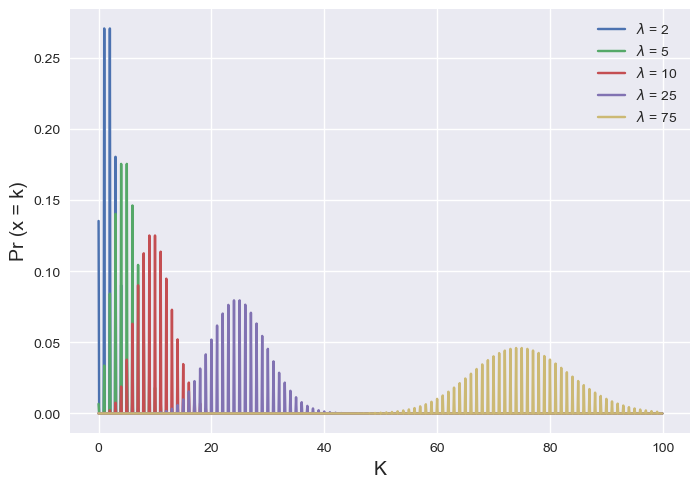
\includegraphics[width=\textwidth]{img/math/poisson.png}
  \caption{Distribuzione cumulativa della variabile di Poisson al variare di $\lambda$ con $T=1$.}
  \label{fig:poisson}
\end{figure}

\begin{figure}[ht]
  \centering
  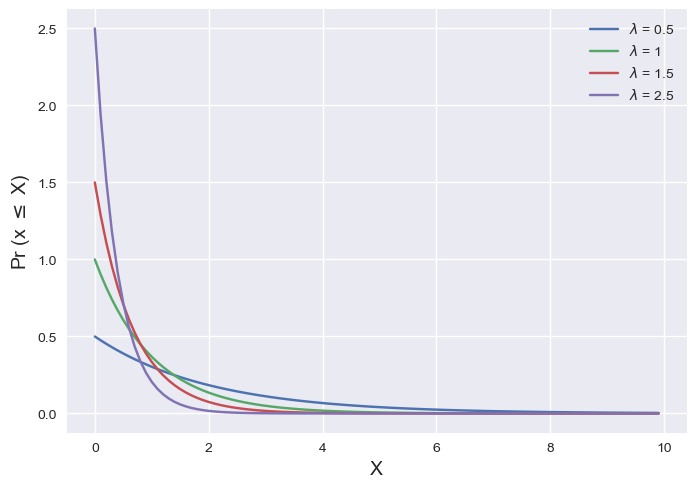
\includegraphics[width=\textwidth]{img/math/exponential.png}
  \caption{Distribuzione di probabilità della variabile esponenziale al variare di $\lambda$.}
  \label{fig:exponential}
\end{figure}

Una importante proprietà della distribuzione di Poisson è la sua relazione con la distribuzione esponenziale (\cref{fig:poisson}). Infatti, così come la distribuzione binomiale esprime il numero di successi in $n$ prove indipendenti (prove di Bernoulli\cite{gelliprobabilita}) e quella geometrica l'intervallo di tempo tra due successi consecutivi, così la distribuzione di Poisson fornisce una stima del numero di eventi in un intervallo finito $T$ e l'esponenziale mette in risalto la distanza temporale tra due eventi consecutivi. Formalmente, questa relazione è messa in evidenza dal tempo di inter-arrivo ($T_a$) tra due eventi che segue un andamento esponenziale\footnote{Si noti che la relazione sussiste tra una variabile aleatoria continua e una discreta}:
\begin{equation}
    Pr\;[T_a < t ] = 1 - e^{-\lambda t}
    \label{eq:cdf}
\end{equation}

Questa proprietà è messa in risalto dal fatto che il tempo di inter-arrivo degli eventi della distribuzione esponenziale coincide con:

\begin{equation}
    E\;[T_a] = \frac{1}{\lambda}
    \label{eq:interarrival}
\end{equation}

mentre il numero medio di eventi al secondo della distribuzione di Poisson è dato dal \textit{rate}:

\begin{equation}
    Mean = \lambda
    \label{eq:rate}
\end{equation}

Pertanto, la relazione che lega la distribuzione di Poisson alla variabile aleatoria esponenziale è la reciprocità tra \textit{rate} di Poisson e tempo di inter-arrivo esponenziale:
\begin{equation}
    E\;[T_a] = \frac{1}{mean}=\frac{1}{\lambda}.
\end{equation}


\subsection{Modello a singola coda}\label{s:mm1}
In base a quanto illustrato in \cref{poisson}, in questo elaborato i tempi di inter-arrivo e di servizio sono assunti casuali e, quindi esponenziali. Secondo la notazione di Kendall, $A=B=M$; mentre utilizzando un solo server $m=1$. Pertanto, il modello utilizzato si chiama a singola coda e viene indicato con $M/M/1$ (schematizzato in \cref{s:mm1}). Di seguito sono mostrati i parametri di \textit{performance} più importanti per i sistemi a singola coda\cite{bolch2006queueing}.

\begin{figure}
  \centering
  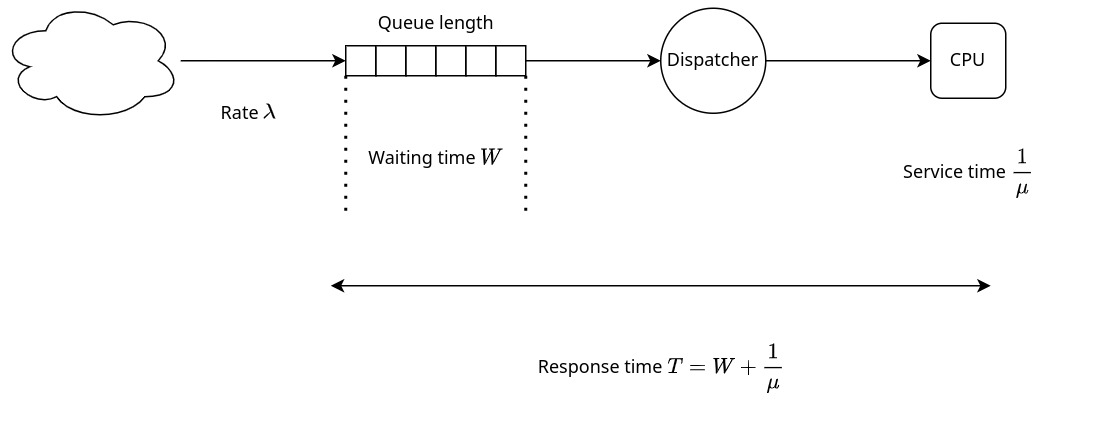
\includegraphics[width=\textwidth]{img/arch/tesi-Pagina-4.jpg}
  \caption{Schema modello a singola coda $M/M/1$.}
  \label{fig:mm1}
\end{figure}


\paragraph{Utilizzazione del processore $\rho$}\cite{bolch2006queueing}
Nei modelli a singola coda, la porzione di tempo per cui il processore risulta occupato dipende dal tempo di inter-arrivo ($\lambda$) dei processi e dal tempo di servizio ($\mu$). In particolare:
\begin{equation}
    \rho = \frac{\lambda}{\mu}
\end{equation}

Inoltre, la condizione per la stabilità per un sistema è $\rho < 1$.

\paragraph{Throughput}

Come accennato in \cref{tab:server_spec}, il \textit{throughput} è una misura per indicare quante richieste vengono servite in un intervallo di tempo. Nei sistemi a singola coda con memoria infinita, il \textit{throghput} è pari a $\lambda$ in quanto nessun processo viene rifiutato. In realtà, questo valore viene saturato in base alla dimensione $K$ del buffer delle richieste e vale la relazione $K \leq n$, con $n$ numero di richieste che arrivano al sistema.

\paragraph{Tempo di attesa}
Il tempo di attesa è il tempo che una richiesta spende nel sistema quando non usufruisce della CPU. In particolare, detto $\overline{T}$ il tempo di risposta (o tempo di residenza), l'intervallo che il processo spende nel sistema, allora si può definire il tempo di attesa $\overline{W}$ come:

\begin{equation}
    \overline{W} = \overline{T} - \frac{1}{\mu}
\end{equation}

\paragraph{Numero di processi nel sistema $K$}
Il numero di processi in un sistema è uno dei più importanti parametri dei sistemi a singola coda e dipende dalla probabilità di avere processi nel sistema $\pi_k$. In particolare, il numero di processi nel sistema può essere espresso come\cite{bolch2006queueing}:
\begin{equation}
    \overline{K} = \sum_{k=1}^{\infty}k\pi_k
\end{equation}

Inoltre, grazie alla legge di Little\cite{wiki:littlelaw}, $\overline{K}$ può essere calcolato come:
\begin{equation}
    \overline{K} =\lambda\overline{T}
\end{equation}
dove con $\overline{T}$ è stato indicato il tempo di risposta medio di una richiesta. Analogamente, la dimensione media della coda $\overline{O}$ può essere espressa, secondo la legge di Little, in funzione del tempo medio di attesa $\overline{W}$:

\begin{equation}
    \overline{O} =\lambda\overline{W}
\end{equation}

\subsection{Stabilità}
Una delle proprietà fondamentali del modello a singola coda è la stabilità. Infatti, con i risultati della teoria di Markov\cite{bolch2006queueing}(capp. 2-3), è possibile studiare il comportamento del modello una volta raggiunta una condizione di regime. Il primo valore che si ricava dagli studi di Markov è la probabilità che la coda sia vuota $\pi_o$:

\begin{equation}
    \pi_0 = \frac{1}{1+\sum\limits_{k=1}^\infty \prod\limits_{i=0}^{k-1} \frac{\lambda}{\mu}} = 1 - \frac{\lambda}{\mu} = 1 - \rho
    \label{equation:pi0}
\end{equation}
Inoltre, si dimostra che la probabilità $\pi_k$ di avere $K$ processi all'interno della coda dipende dall'utilizzazione del processore, come mostrato di seguito:

\begin{equation}
    \pi_k = \pi_0 \left(\frac{\lambda}{\mu}\right)^k
    \label{equation:pik}
\end{equation}

Quindi, ricordando che $\frac{\lambda}{\mu} = \rho$ e sostituendo la \ref{equation:pi0} nella \ref{equation:pik}, si ottiene che:

\begin{equation}
    \pi_k = (1 - \rho)\rho^k
\end{equation}

L'ultima relazione indica che la probabilità del numero di processi all'interno del sistema varia secondo una distribuzione geometrica (il cui andamento è mostrato \cref{fig:geometric}). Pertanto, il numero medio dei processi nel sistema risulta:
\begin{equation}
    \overline{K} = \frac{\rho}{1-\rho}
\end{equation}

\begin{figure}[ht]
  \centering
  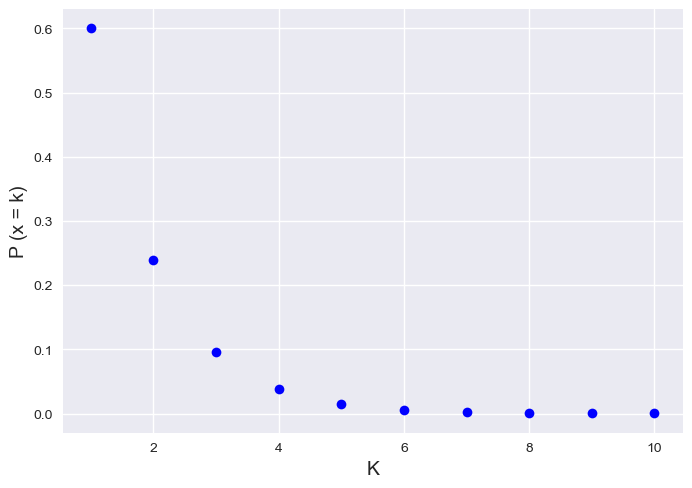
\includegraphics[width=\textwidth]{img/math/geometric.png}
  \caption{Andamento distribuzione geometrica con $\rho=0.6$}
  \label{fig:geometric}
\end{figure}

\section{Architettura client-server}
Nell'esperimento presentato in \cref{ch:esperimento}, è utilizzato il modello architetturale \textit{client-server} in cui sono distinti due tipi di processi:

\begin{itemize}
    \item \textbf{\textit{Server}}: processi che mettono a disposizione dei servizi;
    \item \textbf{\textit{Client}}: processi che fruiscono dei servizi offerti dal server;
\end{itemize}
In questa architettura, il processo \textit{server} resta in attesa di richieste che possono arrivare in maniera concorrente da uno o più \textit{client}. Infatti, sono sempre i \textit{client} ad iniziare la comunicazione con il server, e in generale, una comunicazione può essere composta da un'interazione complessa come nel caso di connessioni TCP.

\chapter{Case study: slow client}\label{ch:case_study}

\section{Descrizione}\label{s:descrizione}

Il \textit{case study} prevede l'analisi delle prestazioni di un \textit{server} che accetta due tipi di richieste:
\begin{itemize}
    \item \textbf{Richieste lente}\footnotemark{}: all'interno di un'applicazione reale, una richiesta lenta può rappresentare operazioni \textit{I/O bound} (connessioni ad un database, richieste a servizi esterni, operazioni su disco etc.) o \textit{CPU bound} (operazioni di crittografia, calcoli matematici avanzati etc.);
    \item \textbf{Richieste veloci}\footnotemark[\value{footnote}]: sono operazioni leggere che richiedono pochi passaggi in memoria (aggiornamento di variabili locali, lettura da cache, operazioni matematiche semplici etc.)
\end{itemize}

\footnotetext{In questo contesto, per "velocità" si intende il tempo medio di esecuzione di un processo ed è relativo alle richieste stesse. Per richieste di velocità diverse, infatti, si indicano processi i cui tempi di esecuzione viaggiano su ordini di grandezza differenti.}

Se non gestiti correttamente, i due flussi in ingresso possono condurre il sistema ad un situazione di \textit{trashing} in cui entrambe le classi di traffico soffrono di \textit{performance} degradate. Infatti, con riferimento ai parametri descritti in \cref{s:mm1}, la gestione inefficiente delle richieste lente comporta un aumento del numero medio di processi nel sistema, con conseguente aumento del tempo medio di risposta (e tempo di attesa) sia delle richieste lente, ma anche di quelle veloci\cite{644616}.\\

Lo scopo dell'analisi è quello di fornire una comparazione delle prestazioni del server utilizzando due algoritmi di \textit{scheduling} differenti: FCFS (\textit{first come first served}) e DRR (\textit{deficit round robin}), In particolare, l'attenzione sarà posta su come variano le \textit{performance} quando, utilizzando DRR, viene data maggiore priorità alle richieste veloci.

\section{Esperimento}\label{ch:esperimento}

L'esperimento prevede la creazione di un'architettura client-server. Il \textit{client} si occupa di orchestrare l'invio di \textit{workload} al server che risponde ad ogni richiesta con le informazioni utili all'analisi delle prestazioni.\\
Al fine di evidenziare il fenomeno di degradazione delle performance, l'esperimento sarà condotto utilizzando connessioni TCP in quanto ciascuna connessione richiede l'allocazione di risorse predicibili che producono delle variazioni significative nei parametri misurati.

\subsection{Metodologie utilizzate}\label{s:metodologie}
In questa sezione, sono descritte le tecniche e le tecnologie utilizzate per condurre l'esperimento.

\subsubsection{Hardware}
Client e server sono due macchine virtuali installate in server diversi con le specifiche tecniche descritte in \cref{tab:server_spec} e \cref{tab:client_spec}.

\begin{table}
    \centering
    \begin{tabular}{|p{2.5cm}||p{9cm}| }
        \hline
         RAM& 1GB, ECC DIMM\\
         \hline
         \hline
         CPU& 1vCPU, 2GHz\\
         \hline
         \hline
         Network& Virtual adapter con driver VirtIO\\
         \hline
         \hline
         OS& Debian 11, kernel 5.10.0-16-amd64\\
         \hline
    \end{tabular}
    \caption{Specifiche tecniche macchina server.}
    \label{tab:server_spec}
\end{table}

\begin{table}
    \centering
    \begin{tabular}{|p{2.5cm}||p{9cm}| }
        \hline
         RAM& 2GB, ECC DIMM\\
         \hline
         \hline
         CPU& 1vCPU, 2.2GHz\\
         \hline
         \hline
         Network& Virtual adapter con driver VirtIO\\
         \hline
         \hline
         OS& Ubuntu 20.04 LTS, kernel 5.4.0-96-generic\\
         \hline
    \end{tabular}
    \caption{Specifiche tecniche macchina client.}
    \label{tab:client_spec}
\end{table}

\subsubsection{Go (Golang)}
Go è un linguaggio di programmazione compilato \textit{general purpose} creato in Google nel 2009. Il linguaggio è dotato di un \textit{runtime} multiprocessore \textit{m:n}\footnote{Con questa notazione si indica che il runtime è in grado di gestire m \textit{task} su n processi di sistema operativo. In generale, Go esegue lo \textit{scheduling} dei \textit{task} effettuando il \textit{multiplexing} su un numero di processi uguale a quello dei processori fisici rilevati.} e di \textit{garbage collector}. Go offre un'implementazione nativa di \textit{Communication Sequential Process} (\textit{CSP}) che, insieme alle \textit{goroutine}, lo rende adatto all'implementazione di sistemi concorrenti e ad eventi. Una \textit{goroutine} è l'implementazione di un \textit{thread} che esegue nello spazio utente\footnote{In altre tecnologie, possono essere indicati con \textit{coroutine}, \textit{light thread} o \textit{green thread}.}. In particolare, la realizzazione dei CSP avviene attraverso strutture dette \textit{channel} che si occupano di far comunicare \textit{goroutine} separate, garantendo una consegna ordinata dei messaggi.
Inoltre, il linguaggio mette a disposizione un'implementazione del costrutto \textit{select} che, analogamente alla \textit{system call} \textit{Linux}, consente di monitorare più \textit{channel} bloccandosi fino a quando \textbf{almeno} uno di questi non riceve un messaggio\footnote{In Go, è disponibile una variante non bloccante di questo costrutto mediante il ramo \textit{default} che viene eseguito immediatamente se nessun \textit{channel} è pronto.}.

\subsubsection{Python}
Python è un linguaggio di programmazione interpretato \textit{general purpose}. In questo elaborato, viene utilizzato principalmente per effettuare l'analisi dei risultati dell'esperimento (\cref{s:risultati}). In particolare, con l'utilizzo delle librerie \textit{pandas}\cite{reback2020pandas} e \textit{matplotlib}\cite{Hunter:2007} vengono manipolati i CSV generati, create delle tabelle \textit{pivot} che mettono in relazione i due algoritmi di \textit{scheduling}, estratte le informazioni desiderate e rappresentate graficamente. Nello specifico, nell'ottica della riproducibilità dell'analisi dei risultati, è stato creato un Jupyter notebook\cite{Giuseppe_tesi_2022}.\\
Inoltre, Python viene utilizzato per la creazione del \textit{workload} descritta in \cref{s:workload}.

\subsection{Creazione del workload}\label{s:workload}
Il \textit{workload} è l'insieme di attività da effettuare sul server e viene generato dallo script in \textit{workload.py}\cite{Giuseppe_tesi_2022}, salvato in un file JSON e passato in ingresso al programma \textit{client}\cite{Giuseppe_tesi_2022} che si occupa di effettuare l'attività di \textit{benchmark} e salvare i risultati su un file CSV. Le singole attività sono caratterizzate dalle seguenti proprietà:
\begin{itemize}
    \item \textbf{slow\_rate}: numero di richieste lente da inviare al secondo. In base al numero di partenza, di fine e un incremento, lo script genera un insieme di valori con incremento fisso;
    \item \textbf{fast\_rate}: numero di richieste veloci da inviare al secondo. L'intervallo generato è analogo a quello delle richieste lente;
    \item \textbf{slow\_percent}: percentuale di richieste lente da inviare in relazione al numero di richieste totali. Analogamente ai precedenti insiemi, anche questo intervallo varia secondo una progressione ad incremento fisso;
\end{itemize}

Una volta creati gli intervalli dei parametri, il \textit{workload} viene generato facendo il prodotto cartesiano degli insiemi ottenuti. 

\section{Implementazione}

Il funzionamento generale dell'esperimento è riassunto in \cref{fig:general}.

\begin{figure}
  \centering
  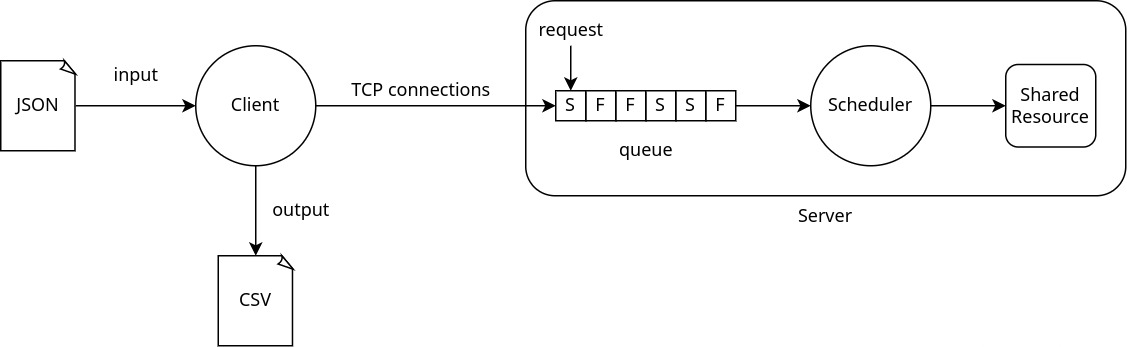
\includegraphics[width=\textwidth]{img/arch/tesi-generale (1).jpg}
  \caption{Schema di funzionamento generale dell'esperimento.}
  \label{fig:general}
\end{figure}

\subsection{Client}
Il client\cite{Giuseppe_tesi_2022} legge da un file una lista di workload e li invia al server. In particolare, il \textit{client} genera una \textit{goroutine} separata per ogni richiesta con una temporizzazione che segue una distribuzione esponenziale (\ref{s:limiti}) e salva le metriche raccolte in un file CSV. Per avere un esperimento più realistico e rendere indipendenti le richieste, il \textit{client} aprirà una nuova connessione per ogni richiesta\footnote{In ogni connessione viene inviata una sola richiesta} e non adotterà alcuna tecnica di \textit{caching} e/o \textit{pooling} delle connessioni che andrebbero a falsare i valori di \textit{round trip time} (RTT, \cref{s:dati}) in quanto verrebbe saltato l'\textit{handshaking} delle connessioni TCP.

\subsection{Server}
Il server\cite{Giuseppe_tesi_2022} si mette in ascolto di connessioni TCP e utilizza una \textit{goroutine} separata per lo \textit{scheduling} delle richieste. L'implementazione dello \textit{scheduling} avviene attraverso il \textit{multiplexing} dei flussi in ingresso in un unico flusso d'uscita, mediante \textit{channel} (\cref{fig:fcfs} e \cref{fig:drr}). Ad ogni richiesta, codificata come un \textit{uint32}\footnote{Il \textit{client} invia $0$ per una richiesta lenta e $1$ per una richiesta veloce}, il server risponde con un documento JSON in cui sono presenti le metriche (\cref{s:dati}) per l'analisi finale.
Al fine di limitare l'ottimizzazione dello \textit{scheduler} interno di Go e di avere risultati realistici, è stato deciso di utilizzare un server con un solo processore fisico (\cref{s:limiti}). L'implementazione\cite{drr_impl} dello \textit{scheduler} DRR è basata sull'algoritmo descritto in \cref{s:drr}.

\begin{figure}
  \centering
  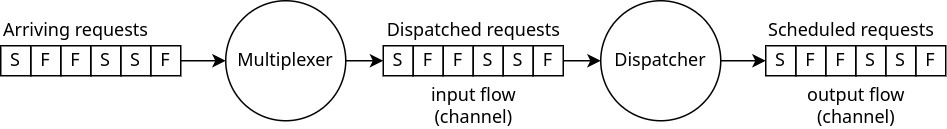
\includegraphics[width=\textwidth]{img/arch/tesi-fcfs.jpg}
  \caption{Implementazione \textit{scheduler} FCFS.}
  \label{fig:fcfs}
\end{figure}

\begin{figure}
  \centering
  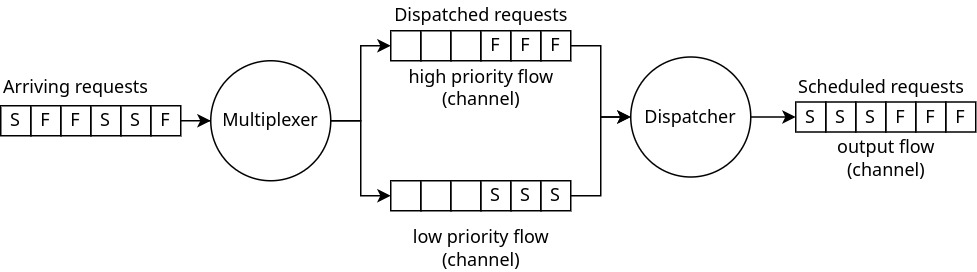
\includegraphics[width=\textwidth]{img/arch/tesi-drr.jpg}
  \caption{Implementazione \textit{scheduler} DRR.}
  \label{fig:drr}
\end{figure}

\section{Raccolta dati}\label{s:dati}

Come accennato in precedenza, per ogni richiesta, il server costruisce una risposta in JSON con i seguenti campi:
\begin{itemize}
    \item \textbf{Istante di accettazione ($I_a$)}: per ogni connessione accettata, il server crea una nuova \textit{goroutine} e, dalla connessione con il client, legge un \textit{uint32} e marca la richiesta come accettata;
    \item \textbf{Istante inizio di esecuzione ($I_e$)}: dopo aver letto il tipo di richiesta, il server ne effettua lo \textit{scheduling}. Quando la richiesta viene schedulata e arriva alla \textit{goroutine} per l'accesso alla risorsa condivisa, la richiesta viene marcata come in esecuzione;
    \item \textbf{Istante di fine esecuzione ($I_f$)}: dopo aver servito la richiesta, viene segnato il tempo di fine esecuzione;
    \item \textbf{Memoria allocata}: insieme al tempo di fine esecuzione viene segnata anche la memoria allocata del sistema al programma server\footnote{Il dato raccolto viene fornito direttamente dal \textit{runtime} e include tutta la memoria allocata dal sistema operativo, insieme allo \textit{stack} e all'\textit{heap} delle singole \textit{goroutine}}.
    \item \textbf{Utilizzazione del processore ($\rho$)}: unitamente alla memoria allocata, nella risposta viene inviato anche l'utilizzazione del processore; 
    \item \textbf{Numero di processi nel sistema ($\overline{K}$)}: assegnando una \textit{goroutine} per ogni connessione ed effettuando esattamente una richiesta per client, il numero di richieste nel sistema corrisponde al numero di \textit{goroutine} escluse quelle già in esecuzione;
\end{itemize}

Con le metriche appena descritte, il \textit{client} calcola le seguenti statistiche:
\begin{itemize}
    \item \textbf{Tempo di residenza medio} ($T_r$): tempo speso dalla richiesta all'interno del sistema. Viene calcolato con $I_f-I_a$;
    \item \textbf{Tempo di attesa medio} ($T_w$): tempo speso dalla richiesta in coda prima di essere servita. Viene calcolato con $I_e - I_a$;
\end{itemize}

Per ogni \textit{workload}, il \textit{client} calcola il valore medio di tutte statistiche illustrate.

\section{Limiti}\label{s:limiti}

\subsection{Misura degli istanti temporali}
Go utilizza uno scheduler \textit{fair} per le sue \textit{goroutine} e, in caso di \textit{system call}, il runtime potrebbe ottimizzare l'operazione con un \textit{context switch}. La presenza di una sola CPU all'interno del server rende possibile un confronto alla pari con altri \textit{runtime} \textit{single-threaded}. 

\subsection{Misurazione utilizzazione del processore}
La misurazione della percentuale di carico della CPU è un'operazione che dipende strettamente dal sistema operativo utilizzato. In questo elaborato, per utilizzazione del processore viene utilizzato il valore medio calcolato nell'ultimo minuto. In particolare, utilizzando un sistema operativo \textit{Linux-based}, questo valore viene letto dal file virtuale \textit{/proc/stat}.

\subsection{Generazione temporizzata degli eventi}
L'implementazione utilizzata per la generazione degli eventi utilizza la funzione \textit{time.After(d time.Duration)}.\\
Quest'approccio presenta due limiti: il tipo \textit{time.Duration} esprime gli intervalli temporali con una precisione del nanosecondo (quindi per \textit{workload} con \textit{rate} molto alti, la risoluzione potrebbe non bastare)\footnote{In Go, il tipo \textit{time.Duration} è un alias per \textit{int64}.}; mentre la funzione \textit{time.After} consegna un messaggio attraverso un \textit{channel} dedicato che non assicura la immediata schedulazione della \textit{goroutine}, ma solo che sia trascorso \textbf{almeno} l'intervallo espresso nel parametro di ingresso.

\section{Risultati}\label{s:risultati}

I risultati presentati di seguito sono stati ottenuti applicando il \textit{workload} descritto in \cref{tab:workload} effettuando $10000$ richieste per blocco. Inoltre, il server serve una richiesta lenta sospendendo l'esecuzione della \textit{goroutine} per un millisecondo.

\begin{table}
    \centering
    \begin{tabular}{|p{3cm}||p{3cm}||p{3cm}||p{3cm}| }
        \hline
        Parametro& Inizio& Fine& Incremento\\
        \hline
         Slow Load & 10 (\%)& 70 (\%)& 20\\
         \hline
         \hline
         Slow rate& 1000 (rps)& 5000 (rps)& 1000\\
         \hline
         \hline
         Fast rate& 1000 (rps)& 5000 (rps)& 1000\\
         \hline
         \hline
    \end{tabular}
    \caption{Parametri utilizzati per generare il \textit{workload}.}
    \label{tab:workload}
\end{table}

\subsection{Analisi richieste lente}
Come anticipato in \cref{s:scheduling}, l'applicazione di un algoritmo a priorità può portare alla \textit{starvation} dei processi a bassa priorità. Infatti, come mostrato in \cref{fig:slow_byslow}, il tempo medio di attesa delle richieste lente è più basso con l'algoritmo FCFS, ma si noti che aumentando la percentuale di carico, le due strategie di \textit{scheduling} tengono a comportarsi allo stesso modo.

\begin{figure}
  \centering
  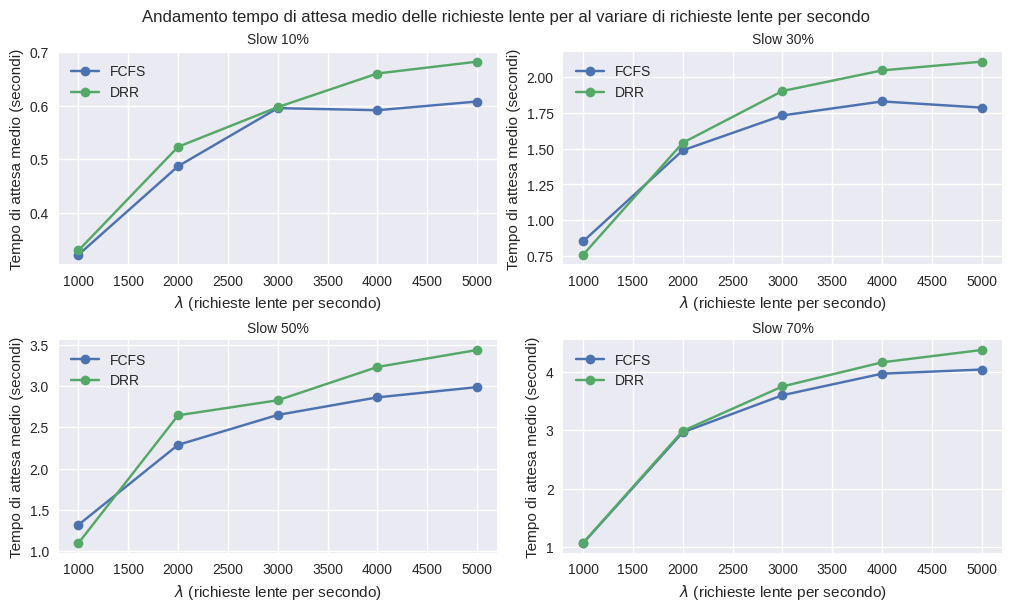
\includegraphics[width=\textwidth]{img/results/slow_wt_byslow.png}
  \caption{Andamento tempo medio di attesa delle richieste lente con variazione del numero di richieste lente per secondo.}
  \label{fig:slow_byslow}
\end{figure}

Inoltre, si noti come facendo variare le richieste veloci, con l'algoritmo DRR, il tempo di attesa delle richieste lente può aumentare del $27\%$ rispetto alla politica FCFS, come mostrato in \cref{fig:slow_byfast}.

\begin{figure}
  \centering
  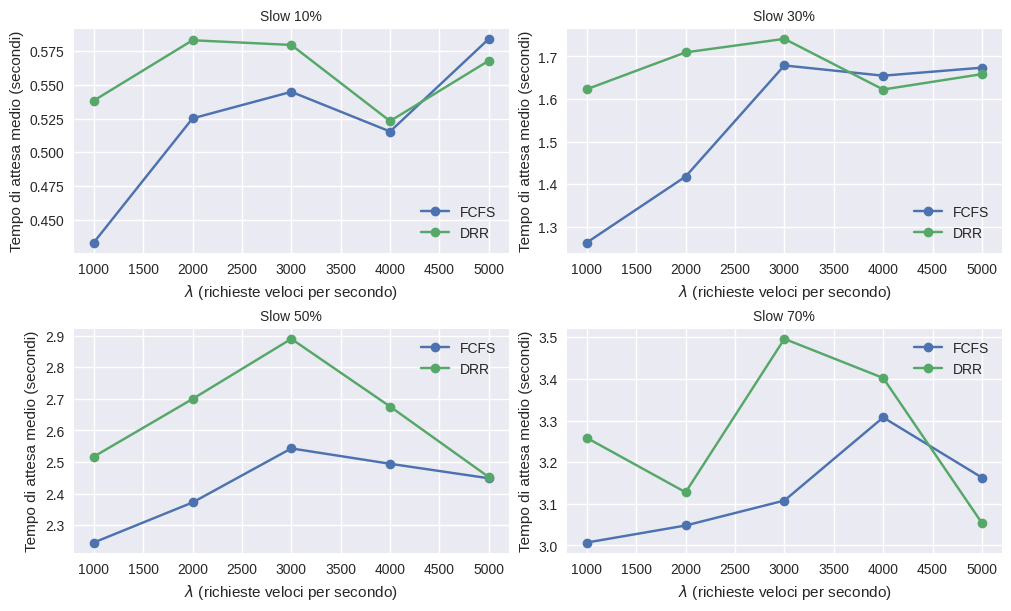
\includegraphics[width=\textwidth]{img/results/slow_wt_byfast.png}
  \caption{Andamento tempo medio di attesa delle richieste lente con variazione del numero di richieste veloci per secondo.}
  \label{fig:slow_byfast}
\end{figure}

\subsection{Analisi richieste veloci}\label{s:fast_an}
Dare una maggiore priorità alle richieste veloci, porta ad un miglioramento generale alle prestazioni del server (\cref{fig:fast_byslow}). Infatti, si noti come ad una crescita pseudo-lineare del tempo di attesa con FCFS, corrisponde un andamento quasi costante con DRR. In particolare, quando il server ha poche richieste lente (\textit{slow=10\%}), DRR risulta sconveniente, ma all'aumentare della frequenza di arrivo si registra un miglioramento dei tempi di attesa di circa il $75\%$; questo miglioramento viene mantenuto anche nel caso in cui il numero di richieste lente è uguale a quelle veloci. Inoltre, il basso tempo di attesa delle richieste veloci contribuisce come illustrato in \cref{s:jobs} a una maggiore capacità del server.

\begin{figure}
  \centering
  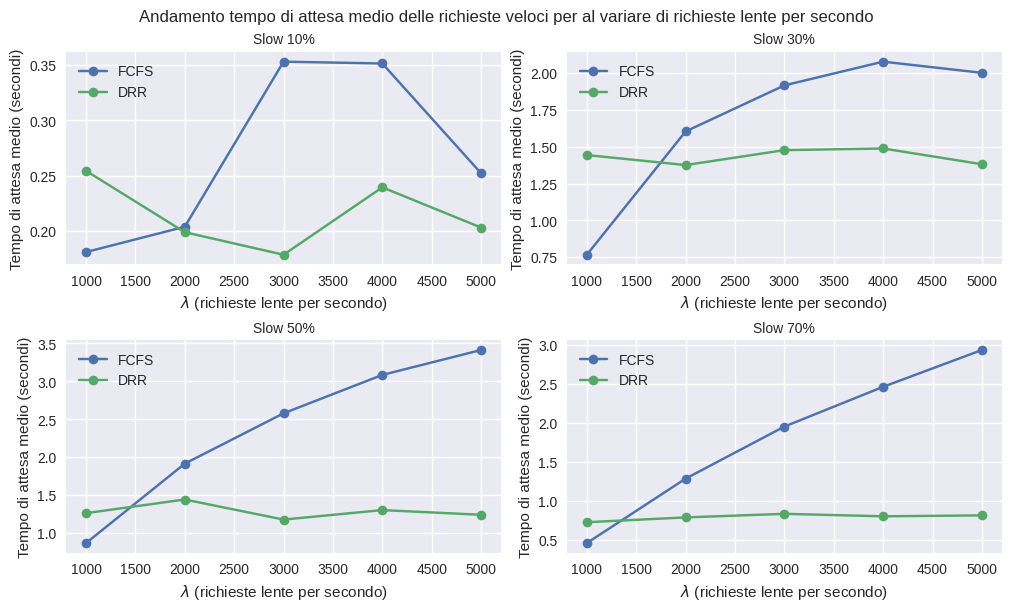
\includegraphics[width=\textwidth]{img/results/fast_by_slow.png}
  \caption{Andamento tempo medio di attesa delle richieste veloci con variazione del numero di richieste lente per secondo.}
  \label{fig:fast_byslow}
\end{figure}

Analogamente, al caso delle richieste lente, osservando come variano i tempi di risposta rispetto alla frequenza delle richieste veloci si evince che i due algoritmi si comportano in modo simile (\cref{fig:fast_byfast}).

\begin{figure}
  \centering
  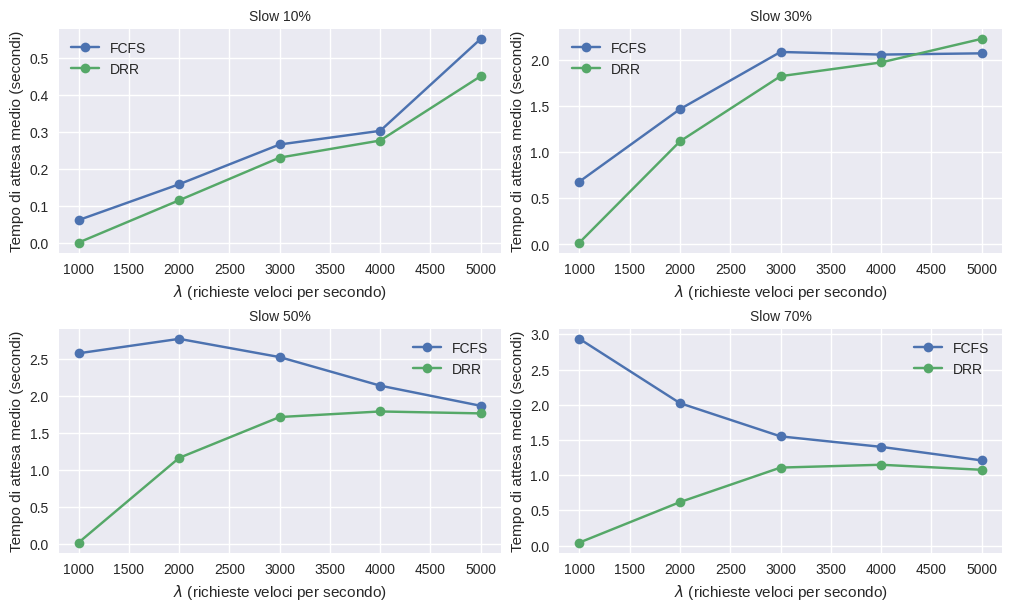
\includegraphics[width=\textwidth]{img/results/fast_byfast.png}
  \caption{Andamento tempo medio di attesa delle richieste veloci con variazione del numero di richieste veloci per secondo.}
  \label{fig:fast_byfast}
\end{figure}

\subsection{Numero di processi nel sistema}\label{s:jobs}
Dall'analisi effettuata in \cref{s:fast_an}, è immediato ricavare che, utilizzando l'algoritmo DRR, il numero di richieste nel sistema si abbassa quando cresce il numero di richieste veloci in quanto vengono servite con priorità maggiore, come mostrato in \cref{fig:jobs}. In particolare, si noti come entrambi gli algoritmi presentano un andamento pseudo-lineare, ma l'algoritmo DRR mostra, anche in presenza di poche richieste veloci (\textit{slow=70\%}), una retta a pendenza minore.


\begin{figure}
  \centering
  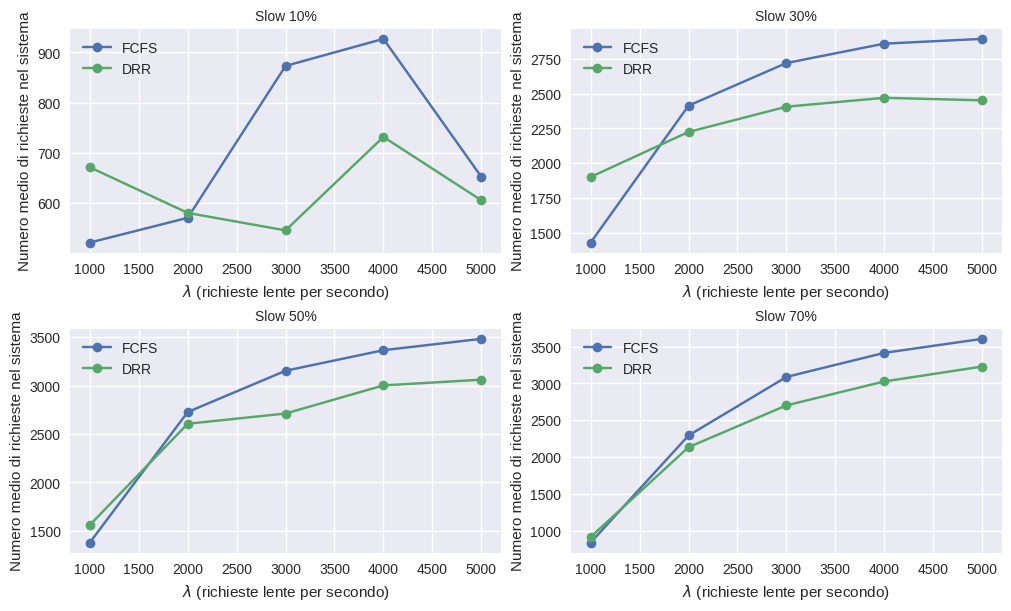
\includegraphics[width=\textwidth]{img/results/jobs.png}
  \caption{Andamento numero medio di richieste nel sistema.}
  \label{fig:jobs}
\end{figure}

\subsection{Utilizzazione CPU}
Dando priorità alle richieste veloci, la CPU spende meno tempo in media in attesa del completamento della richiesta lenta. Infatti, come mostrato in \cref{fig:cpu}, con l'algoritmo DRR, $\rho$ arriva fino al $70\%$; mentre, con FCFS raggiunge il $64\%$ solo con carico di richieste lente al $70\%$ con $\lambda=2000$. Si noti che in ipotesi di numero di richieste lente uguali a quelle veloci ($slow=50\%$), $\rho$ migliora del $30\%$.

\begin{figure}
  \centering
  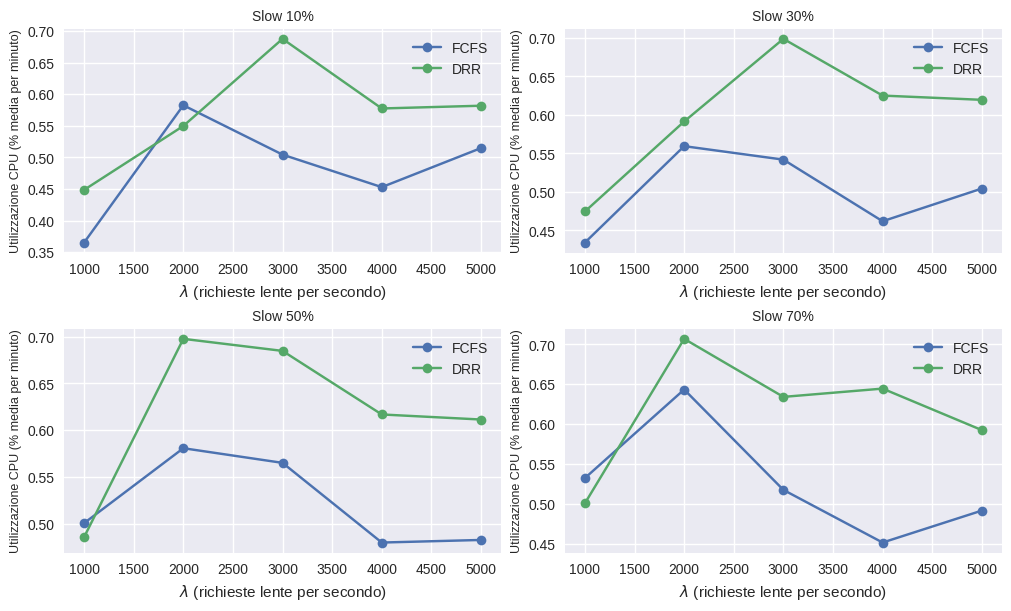
\includegraphics[width=\textwidth]{img/results/cpu.png}
  \caption{Andamento utilizzo processore.}
  \label{fig:cpu}
\end{figure}

\chapter*{Conclusioni}
L'adozione di un algoritmo a priorità nei sistemi con diverse classi di traffico comporta sempre un miglioramento delle prestazioni generali del sistema, e in particolare, del tipo di richieste privilegiate, ma introduce latenze per i le richieste a bassa priorità. Come mostrato nei risultati, la \textit{fairness} di un algoritmo mitiga il fenomeno della \textit{startvation} che non può essere eliminato.

\bibliography{bibliography}
\bibliographystyle{plain}

\end{document}
